% This is samplepaper.tex, a sample chapter demonstrating the
% LLNCS macro package for Springer Computer Science proceedings;
% Version 2.21 of 2022/01/12
%
\documentclass[runningheads]{llncs}
%
\usepackage[T1]{fontenc}
% T1 fonts will be used to generate the final print and online PDFs,
% so please use T1 fonts in your manuscript whenever possible.
% Other font encondings may result in incorrect characters.
%
\usepackage[utf8]{inputenc}
\usepackage[english]{babel}
\usepackage{booktabs}
\usepackage{hyperref}
\usepackage[utf8]{inputenc}
\usepackage[english]{babel}
\usepackage{booktabs}
\usepackage{hyperref}
\usepackage{multicol}
\usepackage{graphicx}
% Used for displaying a sample figure. If possible, figure files should
% be included in EPS format.
%
\usepackage{float}
\usepackage[vlined,algoruled,linesnumbered]{algorithm2e}
\usepackage{amsmath,amssymb,nccmath,mathtools}
\usepackage{tabularx}
\usepackage{siunitx}
\usepackage[vlined,algoruled,linesnumbered]{algorithm2e}
\usepackage{amsmath,amssymb,nccmath,mathtools}
\usepackage{tabularx}
\usepackage{siunitx}
% If you use the hyperref package, please uncomment the following two lines
% to display URLs in blue roman font according to Springer's eBook style:
\usepackage{xcolor}
\renewcommand\UrlFont{\color{blue}\rmfamily}
\urlstyle{rm}
%
%
%
\usepackage{array,multirow,makecell}
\setcellgapes{1pt}
\makegapedcells
\newcolumntype{R}[1]{>{\raggedleft\arraybackslash }b{#1}}
\newcolumntype{L}[1]{>{\raggedright\arraybackslash }b{#1}}
\newcolumntype{C}[1]{>{\centering\arraybackslash }b{#1}}
\usepackage{stmaryrd}

\SetKwRepeat{Do}{do}{while}%

\usepackage{enumerate}
%
%
\begin{document}
%
\title{Masked Computation of the Floor Function and Its Application to the FALCON Signature}
%
\titlerunning{Masked Floor Function For FALCON}
% If the paper title is too long for the running head, you can set
% an abbreviated paper title here
%
\author{Justine Paillet\inst{1,3}\orcidID{0009-0009-6056-7766} \and
  Pierre-Augustin Berthet\inst{2,3}\orcidID{0009-0005-5065-2730} \and
C\'edric Tavernier\inst{3}\orcidID{0009-0007-5224-492X}}
%
\authorrunning{J Paillet et al.}
% First names are abbreviated in the running head.
% If there are more than two authors, 'et al.' is used.
%
\institute{
  Université Jean-Monnet, Saint-\'Etienne, France, \email{justine.paillet@univ-st-etienne.fr}
  \and
  Télécom Paris, Palaiseau, France, \email{berthet@telecom-paris.fr}
  \and
  Hensoldt SAS FRANCE, Plaisir, France, \email{<pierre-augustin.berthet,justine.paillet,cedric.tavernier>@hensoldt.net}
}
%
\maketitle              % typeset the header of the contribution
%
\begin{abstract}

  Falcon is condidate for standardization of the new Post Quantum
  Cryptography (PQC) primitives by the National Institute of Standards
  and Technology (NIST). However it remains a challenge to define
  efficient countermeasures against side channel attacks (SCA). Falcon
  is a lattice-based signature which relies of rational numbers which
  is unusual in the cryptography field. While recent work proposed a
  solution to mask the addition and the multiplication, some
  roadblocks remains, most noticeably how to protect the floor
  function. We propose in this work to complete the existing first
  trials of hardening Falcon againt SCA. We perform the mathematical
  proofs of our methods as well as formal security proof in the
  probing model using the Non-Interference concepts.

  
%With the ongoing standardization of new Post Quantum Cryptography (PQC) primitives by the National Institute of Standards and Technology (NIST), it is important to investigate the robustness of new designs to Side Channel Analysis (SCA). Amongst those future standards is Falcon, a lattice-based signature which relies of rational numbers. It thus requires an implementation using floating point arithmetic, which is harder to design well and secure. While recent work proposed a solution to mask the addition and the multiplication, some roadblocks remains, most noticeably how to protect the floor function. In this work we propose several methods to protect the computation of the floor function. We provide mathematical proofs of our methods as well as formal security proof in the probing model using the Non-Interference concepts. We also discuss their application to the FALCON Signature.
%With the ongoing standardization of new Post Quantum Cryptography (PQC) primitives by the National Institute of Standards and Technology (NIST), it is important to investigate the robustness of new designs to Side Channel Analysis (SCA). Amongst those future standards is Falcon, a lattice-based signature which relies of rational numbers. It thus requires an implementation using floating point arithmetic, which is harder to design well and secure. While recent work proposed a solution to mask the addition and the multiplication, some roadblocks remains, most noticeably how to protect the floor function. In this work we propose several methods to protect the computation of the floor function. We provide mathematical proofs of our methods as well as formal security proof in the probing model using the Non-Interference concepts. We also discuss their application to the FALCON Signature.

\keywords{Floor Function \and Floating-Point Arithmetic \and Post-Quantum Cryptography \and FALCON \and Side-Channel Analysis \and Masking}
\end{abstract}
%
%
%
\section{Introduction}
With the rise of quantum computing, mathematical problems which were
hard to solve with current technologies will be easier to breach and
among the concerned problems, the Discrete Logarithm Problem (DLP)
could be solved in polynomial times by the Shor quantum algorithm
\cite{doi:10.1137/S0036144598347011}. As much of the current
asymmetric primitives rely on this problem and will be breach, new
cryptographic primitves are studied. The National Institute of
Standards and Technology (NIST) launched a post-quantum
standardization process \cite{chen2016report}. The finalists are
CRYSTALS Kyber \cite{8406610,nistfips203mlkem}, CRYSTALS Dilithium
\cite{Ducas_Kiltz_Lepoint_Lyubashevsky_Schwabe_Seiler_Stehlé_2018,nistfips204mldsa},
SPHINCS+ \cite{10.1145/3319535.3363229,nistfips205shdsa} and FALCON
\cite{prest2020falcon}.

\medskip

\noindent Another concern for the security of cryptographic primitives
is their robustness to a Side-Channel opponent. Side-Channel Analysis
(SCA) was first introduced by Paul Kocher
\cite{10.1007/3-540-68697-5_9} in the mid-1990. This new branch of
cryptanalysis focuses on studying the impact of a cryptosystem on its
surroundings. AS computations take time and energy, an opponent able
of accessing the variation of one or both could find correlations
between its physical observations and the data manipulated, thus
resulting in a leakage and a security breach. Thus, the study of
weaknesses in implementations of new primitives and the ways to
protect them is an active field of research.

\medskip 

\noindent While they have been many works focusing on CRYSTALS
Dilithium and CRYSTALS Kyber, summed up by Ravi et
al. \cite{10.1145/3603170}, FALCON is noticeably harder to
protect. Indeed, the algorithm relies on floating-point arithmetic,
for which there is little litterature on how to protect it.
%
\subsubsection{Related Work} Previous works have identified two main weaknesses within the signing process of Falcon: the pre-image computation and the Gaussian sampler, it was proved vulnerable by Karabulut and Aysu \cite{9586131} using an ElectroMagnetic (EM) attack. Their work was later improved by Guerreau et al. \cite{Guerreau_Martinelli_Ricosset_Rossi_2022}. To counter those attacks, Chen and Chen \cite{Chen_Chen_2024} propose a masked implementation of the addition and multiplication of FALCON. However, they did not delved into the second weakness of Falcon, the Gaussian sampler.\newline
The Gaussian sampler is vulnerable to timing attacks, as shown by previous work \cite{10.1007/978-3-662-53140-2_16,10.1145/3133956.3134028,cryptoeprint:2019/478,10.1145/3133956.3134023}. A
isochronous design was proposed by Howe et
al. \cite{10.1007/978-3-030-44223-1_4} to counter those attacks. However, a successful single
power analysis (SPA) was proposed by Guerreau et
al. \cite{Guerreau_Martinelli_Ricosset_Rossi_2022} and further
improved by Zhang et al. \cite{10.1007/978-3-031-30634-1_19}. There is
currently no masking countermeasure for FALCON's Gaussian
Sampler. Existing work \cite{10.1007/978-3-031-07082-2_9} tends to
re-write the Gaussian Sampler to remove the use of floating
arithmetic, thus avoiding the challenge of masking the floor function.
%
\subsubsection{Our Contribution}
In this work we further expand the countermeasure from Chen and Chen \cite{Chen_Chen_2024} and apply it to the Gaussian Sampler. We propose a masking method based on the mantissa truncation to compute the floor function. We discuss the application of this method to masking FALCON.

\medskip

Relying on the previous work of Chen and Chen \cite{Chen_Chen_2024}, we also verify the higher-order security of our method in the probing model. Our formal proofs rely on the Non-Interference (NI) security model first introduced by Barthe et al. \cite{barthe2016strong}.

\medskip

Finally, we provide some performances of our methods and compare them with the reference unmasked implementation and the previous work of Chen and Chen \cite{Chen_Chen_2024}. The implementation is tested on a personal computer with an Intel-Core i7-11850H CPU.
%
\section{Notation and Background}\label{sec:background}
\subsection{Notation}
\begin{itemize}
  \item We denote by $A\backsim B$ the set $A$ excluding the values of set $B$, \emph{id est} $(A\backsim B) \bigcap B = \emptyset $.
  \item For $x\in\mathbb{R}$, we denote the floor function of $x$ by $\lfloor x \rfloor$.
  \item We will use the dot $.$ as the separator between the integer part $i$ and the fractional part $f$ of a real number $x=i.f$.
  \item If $(b_i)$ is a 1-bit Boolean shares for value b, we denote $(-b_i)$ as the 64-bit Boolean shares for $2^{64} - b$. It means that if $b=0$, $(-b_i)$ is a 64-bit boolean shares for $0$, and
  $b=1$, $(-b_i)$ is a 64-bit boolean shares for 0x\textsc{ffffffffffffffff}.   
\end{itemize}
%
\subsection{Diagram Legend}
The following diagrams (Figures \ref{fig:RemoveDec}, \ref{fig:SetExponentZero},\ref{fig:Secfprurshmod}) use the same legend:\begin{itemize}
    \item Probing sets are denoted by $P_i$ or $O$ and are colored in \textcolor{red}{red}.
    \item Simulation sets are denoted by $S_i^j$ and are colored in \textcolor{blue}{blue}.
    \item \emph{t-SNI} gadgets are colored in \textcolor{green}{green}.
    \item \emph{t-NI} gadgets are colored in \textcolor{black}{black}.
\end{itemize}
% 
\subsection{FALCON Sign}
FALCON \cite{prest2020falcon} is a Lattice-Based signature using the
GPV framework over the NTRU problem. In this paper we will focus on
the Gaussian Sampler used in the signature algorithm. For more details
on the key generation or the verification, please refer to the
original paper of FALCON\cite{prest2020falcon}.

\subsubsection{Signature} The signature follows the Hash-Then-Sign strategy. The message $m$ is salted with a random value $r$ and then hashed into a challenge $c$. The remainder of the signature aims at building an instance of the SIS problem upon $c$ and a public key $h$, \emph{id est} finding $\vec{s} =(s_1,s_2)$ such as $s_1 + s_2 h = c$. To do so, the need to compute $\vec{s} = (\vec{t}-\vec{z})\mathbf{B}$, with $\vec{t}$ a pre-image vector and $\vec{z}$ provided by a Gaussian Sampler. Chen and Chen \cite{Chen_Chen_2024} focuses on masking the pre-image vector computation. In this work we intend to mask the Gaussian Sampler. The signature algorithm is detailled in Algorithm \ref{alg:falconsign}.
%
%\begin{algorithm}[H]
%  \caption{FALCON Sign \cite{prest2020falcon}}
%  \label{alg:falconsign}
%\end{algorithm}
%
\subsubsection{Gaussian Sampler}

The Gaussian Sampler is the composition of built from the following functions:

\paragraph{ApproxExp.} This function return $2^{63}\times ccs \times e^{-x}$ and depends of a matrix $C$ defined in page ? of \cite{prest2020falcon}:
%
%C =
%$ \left[\begin{array}{cc}
%     \textsc{0x00000004741183a3}, & \textsc{0x00000036548cfc06},\\
%        \textsc{0x0000024fdcbf140a},& \textsc{0x0000171d939de045},\\
%     \textsc{0x0000d00cf58f6f84},& \textsc{0x000680681cf796e3},\\
%     \textsc{0x002d82d8305b0fea},& \textsc{0x011111110e066fd0},\\
%     \textsc{0x0555555555070f00},& \textsc{0x155555555581ff00},\\
%    \textsc{0x400000000002b400},&\textsc{0x7fffffffffff4800}, \\
%     \textsc{x80000000000000000}&
%\end{array}\right]$


\begin{algorithm}[H]
  \caption{ApproxExp(x,ccs) \cite{prest2020falcon}}
  \KwData{Foating-point values $x\in [0, \ln(2)]$ and $ccs\in [0,1]$}
  \KwResult{An integral approximation of $2^{63}\cdot ccs\cdot \exp(-x)$}
  \small
$y \leftarrow C[0]$\tcp*{$y$ and $z$ remain in $\{0\cdots 2^{63}-1\}$ the whole algorithm} 
  $z \leftarrow \lfloor 2^{63}\cdot x\rfloor$\;
\For{\texttt{i from 1 to 12}}{
  $y\leftarrow C[i] - (z\cdot y)>> 63$\;%\tcp*{$(z\cdot y)$ fits in 126 bits, but we only need the top 63 bits}
}
$z \leftarrow \lfloor 2^{63}\cdot ccs\rfloor$\;
$y\leftarrow (z\cdot y)>>63$\;
\Return{y}\;
\end{algorithm}

\paragraph{BerExp.} This function return $1$ with proba $ccs\times e^{-x}$:

\begin{algorithm}[H]
  \caption{BerExp(x,ccs) \cite{prest2020falcon}}
  \KwData{Foating-point values $x$, $ccs$ $\geq 0$}
  \KwResult{A single bit, equal to 1 with probability $ \approx ccs\cdot \exp(-x)$}
  \small
  $s\leftarrow \lfloor x/\ln(2) \rfloor$ \tcp*{Compute the unique decomposition $x = \ln(2^s)+r $ with $(r,s) \in [0, \ln(2))\times \mathbb{Z}^+$}
  $r \leftarrow x-s\cdot \ln(2)$\;
  $s\leftarrow \min(s,63)$\;
  $z\leftarrow (2\cdot \textsc{ApproxExp}(r,ccs)-1) >> s$\;
  $i\leftarrow 64$\;
  \Do{$((w=0)$ and $(i>0))$}{
      $i\leftarrow i-8$\;
      $w\leftarrow \textsc{UniformBits}(8) - ((z>>i)\:\&\: \textsc{0xff})$\;
  }
\Return{$\llbracket w<0 \rrbracket$}\;
\end{algorithm}
\paragraph{SamplerZ.} The gaussian Sampler:

\begin{algorithm}[H]
  \caption{SamplerZ($\mu$,$\sigma'$) \cite{prest2020falcon}}
  \KwData{Foating-point values $\mu$,$\sigma'$ $\in \mathcal{R}$ such that $\sigma' \in [\sigma_{\min}, \sigma_{\max}]$}
  \KwResult{An integer $z\in\mathbb{Z}$ sampled from a distribution very close to $D_{\mathbb{Z},\mu,\sigma'}$}
  \small
  $r\leftarrow \mu - \lfloor \mu \rfloor$\;
  $ccs \leftarrow \sigma_{min}/\sigma'$\;
  \While{1}{
      $z_0\leftarrow \textsc{BaseSampler()}$\;
      $b\leftarrow \textsc{UniformBits}(8) \: \& \: \textsc{0x1}$\;
      $z\leftarrow b+(2\cdot b -1) z_0$\;
      $x\leftarrow \frac{(z-r)^2}{2\sigma'^{2}} - \frac{z_0^2}{2\sigma_{\max}}$\;
      \If{$\textsc{BerExp}(x, ccs) = 1$}{
           \Return{$z + \lfloor \mu \rfloor $}\;
      }
  }
\end{algorithm}


\bigskip




\begin{algorithm}[H]
  \caption{BaseSampler() \cite{prest2020falcon}}
  \KwData{--}
  \KwResult{An integer $z_0 \in \{0,\cdots, 18\}$ such that $z\sim \chi$} 
  \small
$u \leftarrow \textsc{UniformBits}(72)$\;
  $z_0 \leftarrow 0$\;
\For{\texttt{i from 0 to 17}}{
  $z_0 \leftarrow z_0 + \llbracket u < \textsc{RCDT}[i]\rrbracket$\;
}
\Return{$z_0$}\;
\end{algorithm}

\noindent where RCDT is define in Falcon Specification \cite{prest2020falcon}.

\subsection{Floor Function}\label{subsec:floorfunction}
The floor function is defined as follows:
\begin{definition}\label{def:floorfunction}
  $\forall x \in \mathbb{R}$, the floor function of $x$, denoted by $\lfloor x \rfloor$, returns the greatest integer $z$ such as $z\leq x$.\newline
  $\forall x \in \mathbb{R}$, the truncate function of $x=E.F,(E,F)\in\mathbb{Z}\times\mathbb{N}$, denoted by $truncate(x)$, returns $E$.
\end{definition}
There are several ways of computing the floor function. One
relies on floating-point arithmetic \cite{kahan1996ieee}.
\subsubsection{Binary64 Encoding}
A floating-point is encoded\footnote{Binary64 Standard -- IEEE 754 \cite{kahan1996ieee}} with a sign bit $s$, a 11-bits long exponent $e$ and a 52-bits long mantissa $m$ such as:
\begin{equation}\label{eq:ieee754}
  x\in \mathbb{R}, x = (-1)^s \times 2^{1023-e} \times (1+ m\times2^{-52}).
\end{equation}
\subsubsection{Computing The Floor}\label{sec:computefloor}
Computing the floor function on a floating-point is performed by truncating the
mantissa according to the value of the exponent and of the
sign:
\begin{itemize}
  \item If $e<1023$ then if $s=0$ then $\lfloor x \rfloor = 0$ else $\lfloor x \rfloor = -1$. Indeed,\begin{align}
    (e<1023)\wedge(s=0) &\implies 0\leq x \leq  2^{-1} + m\times2^{-53} < 1 \\
    (e<1023)\wedge(s=1) &\implies 0 > x \geq -2^{-1} + -m\times2^{-53} \geq -1.
  \end{align}
  \item If $e>1074$ then $\lfloor x \rfloor = x$. We have \begin{align}
    e>1074 \implies |x| &= 2^{e-1023} + m\times2^{e-1023-52} \\ &= (2^{e-1023})\in\mathbb{N}^* + (m\times2^{e-1075})\in\mathbb{N} \implies x\in\mathbb{N}^*.
  \end{align}
  The sign bit $s$ only changes "$\in\mathbb{N}$" in "$\in\mathbb{Z}$".
  \item If $1023\leq e \leq 1074$ then we truncate the mantissa $m$ of $x$ and remove its $1074-e$ last bits $m^{[52-(e-1023):1]}$. That way we have \begin{align}
    1023\leq e \leq 1074 \implies x&= 2^{e-1023} + m^{[64:1075-e]}\times 2^{52-(e-1023)+e-1023-52} \\
    &= (2^{e-1023})\in\mathbb{N}^* + (m^{[64:1075-e]})\in\mathbb{N}.
  \end{align}
  However, this only provide $truncate(x)$. To get $\lfloor x \rfloor$, one have to take into account the sign bit $s$. We can rely on the fact that $\forall x\in\mathbb{R}^-\backsim\mathbb{Z}, truncate(x) = \lfloor x \rfloor +1$ and $\forall x \in\mathbb{R}^+, truncate(x) = \lfloor x \rfloor$. Thus, recovering the sign bit allows to properly compute the floor function from the truncate one in this case.
\end{itemize}
\begin{remark}
  To compute the truncate function, one can use the same method but discard the use of the sign. For the first case, \emph{id est} $e<1023$, the result is always $0$.
\end{remark}
This method requires
the use of the exponent and the sign, which are both sensitive values. In this work we propose a method to
perform this truncation in a secure manner.

%
\subsection{Masking}
Masking is a generic countermeasure to SCA at the software level. Instead of processing a sensitive data, it is split in random shares which are processed separately, like in Boolean and Arithmetic masking \cite{mangard2008power}. Masking security can be evaluated thanks to the \emph{t-probing} model, first introduce in \cite{ishai2003private}. A gadget is then said secured against \emph{t-}order attacks if no information can be recovered by any set of \emph{t} intermediate values. However, for the composition of gadgets we use a stronger model introduced in \cite{barthe2016strong}: the (Strong) Non-Interference model.
\begin{definition}
  (\emph{t-}Non Interference (\emph{t-NI}) security). A gadget is said \emph{t-}Non Interference (\emph{t-NI}) secure if every set of \emph{t} interemediate values can be simulated by no more than \emph{t} shares of each of its inputs.
\end{definition}
\emph{t-NI} gadgets composition does not imply \emph{t-NI} security. We need a stronger definition for this:
\begin{definition}
  (\emph{t-}Strong Non Interference (\emph{t-SNI}) security). A gadget is said \emph{t-}Strong Non Interference (\emph{t-SNI}) secure if for every set of $t_I$ of internal intermediate values and $t_O$ of its output shares with $t_I + t_O \leq$\emph{t}, they can be simulated by no more than $t_I$ shares of each of its inputs.
\end{definition}

We will use those models in Section \ref{sec:security} to demonstrate the security of our design.

\section{Masking the Floor Function}
In Section \ref{sec:computefloor} we describe how to compute the floor using floating-point arithmetic. In this section we will present masking gadgets to do this feat in a secure manner. We rely on existing gadgets and propose new ones, as shown in Table \ref{tab:gadgets}. 
\begin{table}[ht]
  \label{tab:gadgets}
  \caption{List of gadgets, their security and their reference}
  \begin{tabular}{C{2.5 cm} || C{5.8 cm} C{1.4cm} C{2cm}}
    \toprule
     \textbf{Algorithm} & \textbf{Description} & \textbf{Security} & \textbf{Reference}\\
      \midrule
       SecAnd   & AND of Boolean shares             & \emph{t-SNI} &  \cite{ishai2003private}, \cite{barthe2016strong}\\
       SecAdd         & Addition of Boolean shares        & \emph{t-SNI}&  \cite{coron2015conversion}, \cite{barthe2018masking}\\
       A2B            & Arithmetic to Boolean conversion  & \emph{t-SNI}& \cite{schneider2019efficiently}\\
       B2A            & Boolean to Arithmetic conversion  & \emph{t-SNI}&  \cite{bettale2018improved}\\
       RefreshMasks   & $t$-NI refresh of masks           & \emph{t-NI}&  \cite{barthe2016strong}, \cite{bettale2018improved}\\
       Refresh        & $t$-SNI refresh of masks          & \emph{t-SNI}& \cite{barthe2016strong}\\
       SecOr          & OR of Boolean shares              & \emph{t-SNI}&  \cite{Chen_Chen_2024}\\
       SecNonZero     & NonZero check of shares           & \emph{t-SNI}&  \cite{Chen_Chen_2024}\\
       SecFprUrsh     & Right-shift with sticky bit   & \emph{t-SNI}&  \cite{Chen_Chen_2024}\\
       SecFprNorm64   & Normalization to $[2^{63},2^{64})$ & \emph{t-NI}& \cite{Chen_Chen_2024}\\
       SetExponentZero& Set exponent to zero & \emph{t-SNI} &  Algorithm \ref{algo:SetExponentZero_floor}\\
       SecFprUrshMod & Right-shift without sticky bit & \emph{t-SNI} &  Algorithm \ref{algo:SecFprUrsh}\\
       RemoveDecimal & Truncate the mantissa & \emph{t-SNI} &  Algorithm \ref{algo:RemoveDecimal_floor}\\
       SecBaseInt & Compute the floor & \emph{t-SNI} &  Algorithm \ref{algo:SecFprBaseInt}\\
      \bottomrule
  \end{tabular}  
\end{table}
\begin{remark}
  With small modifications, our design can also be used to compute the truncate and the rounding functions in a secure manner. As only the floor is required to protect FALCON, we will provide the pseudocodes for truncate and rounding in Appendix \ref{app:function}.
\end{remark}

\section{Masking The Floor Function}\label{sec:maskfloor}
In this part we denote by f as one of these three funtions : floor, truncature and round. Differences will be discussed when necessary.

\subsection{Overview}
  %\paragraph[short]{Binary64 -- IEEE 754.} 
  Recall that we're working with floating-point using the Binary64 -- IEEE 754 \cite{kahan1996ieee} standard representation. Its encoding is defined as follows:
    Let $x \in \mathbb{R}$. $x$ is represented by a tuple of three elements $(s,e,m)$, where $s$ is a 1-bit sign, $e$ a 11-bit exponent and $m$ a 52-bit mantissa such as:%\begin{equation}\label{eq:ieee754}x= (-1)^s \times 2^{e-1023} \times (1+m\times 2^{-52})\end{equation}. We have the following Lemma:
    \begin{lemma}
      \label{lemma:function}
      Let f be floor or truncate or rounding.Computing f mainly depends on the exponent $e$, with three different cases:
    \begin{enumerate}
        \item If $e-Zero_\text{f}<0$, then $\text{f}(x)=0$. $Zero_\text{f}$ depends on f. For f= floor or truncate, we take $Zero_\text{f}=1023$. For f=rounding we take $Zero_\text{f}=1022$.
        \item If $e-1075\geq0$, then $\text{f}(x)=x$;
        \item If $0\leq e-Zero_\text{f} \leq 51$,the result must be computed by removing the $52-(e-Zero_{f})$ decimals from $x$ depending on f. 
    \end{enumerate}
    \end{lemma}
    \begin{proof}
      \begin{enumerate}
        \item \textbf{$e-Zero_\text{f}<0$}. This case covers $x\in(-1;1)$ According to Equation \ref{eq:ieee754} we have for $Zero_\text{f}=1023$:\begin{equation}\label{eq:zerof1023}|x|=  2^{e-1023} \times (1+m\times 2^{-52})\leq 2^{-1}\times (1+m\times 2^{-52})<1.\end{equation} Hence $\text{floor}(x)=\text{truncate}(x)=0$. For $Zero_\text{f}=1022$, we have: \begin{equation}\label{eq:zerof1022}|x|=  2^{e-1023} \times (1+m\times 2^{-52})\leq 2^{-2}\times (1+m\times 2^{-52})<0.5.\end{equation} Hence $\text{rounding}(x)=0$.
        \item \textbf{$e-1075\geq0$}. This case covers $x\in\mathbb{Z}$According to Equation \ref{eq:ieee754} we have:\begin{equation}\label{eq:1075}|x|= 2^{e-1023} \times (1+m\times 2^{-52})\geq 2^{52}\times (1+m\times 2^{-52})\geq 2^{52} + m \in\mathbb{N}.\end{equation}Hence $\text{f}(x)=x\in\mathbb{Z}$.
        \item The last case is function specific but covers $x\in\mathbb{R}\backsim(-1;1)\backsim\mathbb{Z}$.
      \end{enumerate}\hfill $\qed$ 
    \end{proof}

    
    These three distinguished cases provide a fixed structure shown in \autoref{algo:SecFprBaseInt} for $f$. We must compute securely all the checks on masked values, and to change in consequence our mantissa, exponent and eventually our sign bit. 

    \subsection{Masked Floor Function}
    The function SecFprBaseInt is the main function to compute masked floor, masked truncature or masked round. Its result depends on the inputed function: gadgets and Zero$_f$ are different. 
    \begin{figure}[!ht]
        \centering
        \includegraphics[width=0.5\textwidth]{figure/secpfrhierarchie.pdf}
        \label{fig:hierar}
        \caption{SecFprBaseInt and its gadgets}
    \end{figure}

    In this subsection, suppose $f$ = floor. We will first present the main structure and then present the gadgets. Gadgets from trunc and round function can be found in annexe (the little differences between gadgets will be explain too):
    \begin{itemize}%[label = $\bullet$]
        \item SetFprExtract;
        \item RemoveDecimal$_\text{trunc}$ and SetExponentZero$_\text{trunc}$;
        \item RemoveDecimal$_\text{round}$ and SetExponentZero$_\text{round}$.
    \end{itemize}
    The particularity of our shift method for calculating floor function is that it requires the gadgets proposed by Chen and Chen \cite{Chen_Chen_2024}. So by proposing this method, we are extending their work to mask the Gaussian sampler by using only the gadgets of their creation.
    By way of summary, we propose a table showing the functions used to create our gadgets and the sources from which they come.

    \begin{figure}[!ht]
        \begin{center}
            \begin{tabular}{C{2.5 cm} || C{6 cm} C{1.2cm} C{2cm}}
              \toprule
               \textbf{Algorithm} & \textbf{Description} & \textbf{Security} & \textbf{Reference}\\
                \midrule
                 SecAnd   & AND of Boolean shares             & $t$-SNI &  \cite{ishai2003private}, \cite{barthe2016strong}\\
                 SecAdd         & Addition of Boolean shares        & $t$-SNI&  \cite{coron2015conversion}, \cite{barthe2018masking}\\
                 A2B            & Arithmetic to Boolean conversion  & $t$-SNI& \cite{schneider2019efficiently}\\
                 B2A            & Boolean to Arithmetic conversion  & $t$-SNI&  \cite{bettale2018improved}\\
                 RefreshMasks   & $t$-NI refresh of masks           & $t$-NI&  \cite{barthe2016strong}, \cite{bettale2018improved}\\
                 Refresh        & $t$-SNI refresh of masks          & $t$-SNI& \cite{barthe2016strong}\\
                 SecOr          & OR of Boolean shares              & $t$-SNI&  \cite{Chen_Chen_2024}\\
                 SecNonZero     & NonZero check of shares           & $t$-SNI&  \cite{Chen_Chen_2024}\\
                 SecFprUrsh     & Right-shift keeping sticky bit updated  & $t$-SNI&  \cite{Chen_Chen_2024}\\
                 SecFprNorm64   & Normalization to $[2^{63},2^{64})$ & $t$-NI& \cite{Chen_Chen_2024}\\
                \bottomrule
            \end{tabular}
        \end{center}
    \end{figure}

    
      \subsubsection{SecFprBaseInt$_\text{f}$ -- \autoref{algo:SecFprBaseInt}}
      We present a global structure for all three functions f = floor/round/truncate.

      \begin{algorithm}[H]
        \caption{SecFprBaseInt$_\text{f}$(x)}
        \label{algo:SecFprBaseInt}
        \KwData{64-bit boolean shares $(x_i)_{1\leq i \leq n}$ for value x }%\\
        %A function f : floor, round or trunc.}
        \KwResult{64-bit boolean shares $(y_i)_{1\leq i \leq n}$ for mantissa value y = f(x).} 
        $((my_i), (ey_i), (sy_i)) \leftarrow$ SecFprExtract($(x_i)$)\;%\tcp*{extract mantissa, exponent and sign}
        $(cx_i) \leftarrow (ey_i)$\;
        $cx_1 \leftarrow ey_1 - \text{Zero}_f$\;%\tcp*{$\text{Zero}_f$ = 1023 for floor }%and trunc, $\text{Zero}_f$ = 1022 for round}
        $(c_i) \leftarrow$ A2B($(cx_i^{(16)})$)\; 
        Refresh($(cx_i)$)\;
        $(my_i) \leftarrow$ SecAnd($(my_i), (\neg(-c_i))$)\;%\tcp*{if c = 0,  my = mx and if c = 1, my = 0 }
        $(my_i), (ey_i), (Rnd_i) \leftarrow$ RemoveDecimal$_f((my_i), (ey_i), (sy_i), (cx_i)$)\;% \tcp*{depends on f}
        $(my_i), (ey_i) \leftarrow$ SecFprNorm64($(my_i),(ey_i)$)\;
        $(my_i) \leftarrow (my_i >> 11)$\;
        $(my_i) \leftarrow$ $(my_i^{[52:1]}) $\;
        $ey_1 \leftarrow ey_1 + 11$\;
        $(ey_i), (sy_i) \leftarrow$ SetExponentZero$_f((ey_i), (\neg(-c_i)), (s_i), (Rnd_i))$\;%\tcp*{set ey at 0 if f(x)=0}
        $(y_i^{(64)}) \leftarrow (sy_i) $\;
        $(y_i^{[63:53]}) \leftarrow (ey_i) $\;
        $(y_i^{[53:1]}) \leftarrow (my_i) $\;
      \Return{$(y_i)$}\;
      \end{algorithm}
      As explained in overview, these three functions can be summarised in a global structure. 
      What will differentiate the three functions will in fact be the gadgets and the Zero$_f$ parameter.
      To perform the floor function, we first extract the data from the encoding and place it in three variables $s_y, e_y$ and $m_y$, which will be linked directly to the output of the algorithm. 
      By extracting this data\footnote{Pseudo-code in appendix: SecFprExtract -- \autoref{algo:SecFprExtract }}, we carry out a few operations on the mantissa and the exponent to match the conventions of Chen's implementation.
        Indeed, the input $x$ is a 64-bit boolean share, consequently we'll have to transform the exponent into a 16-bit arithmetic share by performing a boolean to arithmetic conversion.
        Another important thing to add is the bit implicit in the mantissa. 
        This bit which is not present in the $x$ information, in order to save one bit and gain in precision, is nevertheless very important.
        In particular, it enables us to normalise our shares correctly.
        Once these changes have been made, we can start working on the exponent.

        The first step consists of checking whether the result is an obvious zero or not.
        To do so, we compare $e_y$ and Zero$_f$ -- which is the correponding exponent to  $1=2^0$ -- by calcultating $c_x = e_y - \text{Zero}_f$.
        If $cx$ is negative, $\mid x \mid <1$ and all decimals can be removed by putting $my = 0$.
        We just need to be carefull at the end of the algorithm because of some particular cases\footnote{For example, if $-1<x<0$, we need to return encoding -1, not zero.}.
        This step without taking care of particular case corresponds in reality to the truncature.
        Otherwise, the $m_y$ mantissa will remain unchanged to be adjusted during the next steps.

        A mathematical explanation of Zero$_f$'s choice can be summurize in a few simple calculus.
        In case $f$ = floor or trunc, Zero$_f = 1023$.
        Indeed if $e_y -1023 <0$, $$2^{e_x-1023} \times (1+m_x\times 2^{-52})\quad\leq \quad 2^{-1} \times (1+m_x\times 2^{-52}) \quad< \quad 1$$ 
        We remark a difference for $f$ = round.
        The main reason of this difference is that we want to avoid to reject the case where the binary decomposition of $x$ contains a $1$ at indices $2^{-1} = 0.5$, 
        since we will no longer be able to round off the final result.
        This justify the choice of  Zero$_f =1022$ for rounding function.
        This time, if $e_y -1022 <0$: 
        $$2^{e_x-1023} \times (1+m_x\times 2^{-52})\quad\leq \quad 2^{-2} \times (1+m_x\times 2^{-52}) \quad< \quad 0.5$$ 
        
        To sum up, after the first step, only $my$ can change. The two values it can take are $my$ it-self (no changes) or $0$.
        The second step removes the decimals by shifting them to the right, using RemoveDecimal -- \autoref{algo:RemoveDecimal_floor}. 
        As this algorithm does not normalise the mantissa, we then apply the SecFprNorm64 function, !!!!!!!! followed by a refresh (SecFprNorm64 is a $t$-NI gadgets) and !!!!!!!!!!! a computation of shifted $my$ and $ey$ to set the mantissa back to bits $[52:1]$ and update $ey$.
        Finally, the last step in the algorithm, before reformatting the initial encoding, is to apply the specific encoding of "0" if this is the result to be returned.
        To do this, we apply the SetExponentZero$_f$ function -- \autoref{algo:SetExponentZero_floor}. 
        \begin{algorithm}
            \caption{RemoveDecimal$_{\text{floor}}((my_i), (ey_i), (sy_i), (cx_i))$}
            \label{algo:RemoveDecimal_floor}
            \KwData{64-bit boolean shares $(my_i)_{1\leq i \leq n}$ for mantissa value my; \\
            16-bit arithmetic shares $(ey_i)_{1\leq i \leq n}$ for exponent value ey; \\
            1-bit boolean shares $(sy_i)_{1\leq i \leq n}$ for sign value sy\\
            16-bit arithmetic shares $(cx_i)_{1\leq i \leq n}$ for value cx = ex-2013.}
            \KwResult{64-bit boolean shares $(my_i)_{1\leq i \leq n}$ for mantissa value $my >> (52 - cx)$; \\
                      16-bit arithmetic shares $(ey_i)_{1\leq i \leq n}$ for exponent value $ey +(52 - cx)$;} 
            $cx_1 \leftarrow cx_1 - 52$\;%\tcp*{check if 0$\leq$c$<$51}
            $(c_i) \leftarrow$ A2B($(cx_i)$)\;
            $(cp_i) \leftarrow (c_i^{(16)})$\;
            $(cp_i) \leftarrow$ SecNonZero($cp_i$)\;
            $(c'_i) \leftarrow (- cp_i)$\;%\tcp*{if cp = 0 cx = 0. if not cx = cx }
            $(c_i) \leftarrow$ SecAnd($(c_i), (c'_i)$)\;
            $(cx_i) \leftarrow$ B2A($(c_i)$)\;
            $(cd_i) \leftarrow (-cx_i)$\;
            $(my_i), (rot_i) \leftarrow$ SecFprUrsh$_f$($(my_i), (cd_i)$)\;%\tcp*{$my >> 52 - cx$ and $rot = my^{[52-cx:1]}$}
            $(b_i) \leftarrow$ SecNonZero($(rot_i)$)\;%\tcp*{if $b=0$, $x \in \mathbb{N}$, else $x\in \mathbb{R}/\mathbb{N}$ }
            $(cp_i) \leftarrow$ SecAnd($(cp_i), (sy_i)$)\; 
            $(cp_i) \leftarrow$ SecAnd($(cp_i), (b_i)$)\; 
            $(my_i)\leftarrow$ SecAdd($(my_i), (cp_i)$)\;%\tcp*{add 1 only if $s = 1$ and if $x \in \mathbb{R}/\mathbb{N}$}
            $(ey_i) \leftarrow (ey_i + cd_i)$\; 
          \Return{(Refresh$(my_i)$, Refresh$(ey_i))$}\;
          \end{algorithm}
    \subsubsection{RemoveDecimal$_\text{floor}$ -- \autoref{algo:RemoveDecimal_floor}}
    As we explained at the beginning of this section, we need to remove the decimals from the input number.
    After checking a first result, the mantissa is equal to 0, if $e-\text{Zero}_f<0$, or has remained unchanged.
    This leaves us with the case where a shift is needed. To do so, we write $cx = e - 1023$ as the shift to be performed.
    The case where $cx<0$ has already been treaten by modifying (or not) the mantissa, whatever shift is made, we would have $0>>cx = 0$.
    If $cx=\geq52$, $x$ is already in the correct form. In fact, we have : 
    $$\mid (-1)^s \times 2^{cx} \times(1+m\times 2^{-52})\mid \quad \geq \quad 2^{52} \times(1+m\times 2^{-52})\quad = \quad2^{52} + m \in \mathbb{N}$$
    To avoid removing information if it isn't needed, we replace $cx$ by $0$.
    Be careful if we want to round a number : it's important to compare $cx$ to $53$ instead of $52$. The reason is that we first subtract to $ey$ $1022$ instead of $1023$ when we were checking is the result was 0 or not. So here we need to add 1.
    If $0\leq e_y - 1023 \leq 51$, we need to modify the mantissa to remove -- if necessary-- the decimals.
    Remarks that even in this case, the mantissa can be in the good format. For example if $x = 5$, we have $0\leq e_y-1023 = 1025-1023 = 2 \leq 51$ and $x$ is an integer.
    
    After verifying is $x$ is or isn't a "big" number, i.e. without decimal in its representation, we can shift\footnote{
    In pseudo-code the subtraction is implicite due to the format of a masked value.} $my$ by $cd=52-cx$ by applying a modified \footnote{If
    we want to use Chen's algorithm, it's possible. We just need to compute one shift less then described in our algorithm and then compute an extra shift manually. The disadvantges of using it, is that you need to check if $cx$ is different from $0$ 
    -- to not compute a shift if it isn't needed -- and the cost of computing the sticky bit.} SecFprUrsh$_f$ -- \autoref{algo:SecFprUrsh}: 
    we don't want to keep the sticky bit, so we just removed this part.
    We had an extra output, returning the part we removed.
    Shift a value is a good thing, but that's not exactly the floor function. After this step we just have the truncature.
    When $x$ positive there's no problem at all, floor function is equal to truncature. But when $x$ is negative there is one. It cames from floor properties. Indeed if $x<0$ : 
    \begin{equation}
        \label{eq:floorneg}
        \text{floor}(-x)  = \Bigg\{ \begin{array}{cc}
            \text{trunc}(-x) &  \text{if } x\in\mathbb{N}\\
            \text{trunc}(-x) -1 &  \text{if } x\in\mathbb{R}/\mathbb{N}
         \end{array}
    \end{equation}

    On one hand, checking if $x$ is negative is quite easy : we just have to take a look at if $sy$ is equal to 1.
    On the other hand, checking that $x$ is an integer is trickier. This is where the second modification to SecFprUrsh$_f$ comes in handy. As this function performs a rotation, the bit information is retained until a mask is applied to calculate the shift. 
    We therefore decided to invert the mask in order to retain the suppressed information. If this information has zero Hamming weight
    then $x$ is an integer. We can then use the SecNonZero gadget on this information, which will return $0$ if $x$ is an integer, and 1 if not.
    We denote this result $b=$ SecNonZero(($my_i^{[52 - c_x:1]}$)). 
    In the following truth table (\autoref{figure:flooradjust}) if the result $cp = $ $s\wedge b$ is $1$, the mantissa must be changed.
    \begin{figure}
        \begin{center}
            \begin{tabular}{C{0.5cm} C{0.5cm} || C{3 cm} L{3cm}}
              \toprule
                 $sy$ & $b$ &$cp$ = $sy \wedge b$ & Interpretation\\
              \midrule 
                0 & $b$ & 0 & Positive number\\
                1 & 0  & 0 & $x$ is an integer\\
                1 & 1  & 1 & Negative real\\
              \bottomrule
            \end{tabular}
        \end{center}
        \caption{$cp$ = $sy\wedge b$ truth table and interpretation}
        \label{figure:flooradjust}
    \end{figure}
    Another question is now : how to subtract $s$ from the mantissa if the mantissa is always positive? 
    The sign of $x$ is only define by $sy$, so $\mid x\mid = 2^{ey-1023}\times(1 + my\times 2^{-52})$.
    We already know that if $x$ is positive or an integer,$my = my \pm 0 = my \pm cp$.
    Now let's focus on $x$ a non integer negative number. Let $x$ be a positive real, from \autoref{eq:floorneg}, we can write :
    \begin{equation}\label{eq:floorabs}
        my =\: \mid \text{floor}(-x)\mid \:=\: \mid \text{trunc}(-x) - 1\mid
    \end{equation}
    By using $\mid \text{trunc}(-x) \mid \:=\: \mid -\text{trunc}(x)\mid \:$, we can transform \autoref{eq:floorabs} :
    \begin{equation}\label{eq:floorabs2}
        my =\: \mid \text{floor}(-x)\mid \:=\: \mid -\text{trunc}(x) - 1\mid \:=\: \mid \text{trunc}(x) + 1\mid \:= my + cp
    \end{equation}
    \begin{algorithm}
      \caption{SecFprUrsh$_{\text{floor}}((my_i), (cx_i))$}
      \label{algo:SecFprUrsh}
      \KwData{ 6-bit arithmetic shares $(cx_i)_{1\leq i \leq n}$ for value cx; \\
      64-bit boolean shares $(my_i)_{1\leq i \leq n}$ for sign value $my$.}
      \KwResult{64-bit boolean shares $(my'_i)_{1\leq i \leq n}$ for value $my>>cx$\\
      64-bit boolean shares $(rot_i)_{1\leq i \leq n}$ for value $my^{[cx : 1]}$.} 
        $(m_i)_{1\leq i \leq n} \leftarrow ((1<<63), 0, \cdots, 0)$\;
        \For{\texttt{i from 1 to n}}{
          Right-Rotate $(my_i)$ by $cx_j$\;
          $(my_i) \leftarrow$ RefreshMasks($(my_i)$)\;
          Right-Rotate $(m_i)$ by $cx_j$\;
          $(m_i) \leftarrow$ RefreshMasks($(m_i)$)\;
        }
        $len \leftarrow 1$\;
        \While{$len\leq 32$}{
          $(m_i) \leftarrow (m_i \oplus (m_i>>len))$\;
          $len \leftarrow len<<1$\;
        }
        $(my'_i) \leftarrow$ SecAnd($(my_i), (m_i)$)\;
        $(m_i) \leftarrow (\neg(m_i))$\;
        $(rot_i) \leftarrow$ SecAnd($(my_i), (m_i)$)\;
    \Return{$((my'_i), (rot_i))$}\;
    \end{algorithm}
    From this, we only have to compute a secure addition between $cp$ and $my$.
    The last step of this algorithm is to add the shift $cd$ to $ey$ to keep this data update.
    \begin{algorithm}
        \caption{SetExponentZero$_{\text{floor}}((ey_i), (sy_i), (b_i))$}
        \label{algo:SetExponentZero_floor}
        \KwData{ 16-bit arithmetic shares $(ey_i)_{1\leq i \leq n}$ for exponent value ey; \\
        1-bit boolean shares $(sy_i)_{1\leq i \leq n}$ for sign value sy\\
        64-bit boolean shares $(b_i)_{1\leq i \leq n}$.}
        \KwResult{16-bit boolean shares $(ey_i)_{1\leq i \leq n}$ for exponent value $ey +(52 - cx)$;\\
                  1-bit boolean shares $(sy_i)_{1\leq i \leq n}$ for sign value.} 
        
          $(ey_i) \leftarrow$ A2B($(ey_i)$)\;
          $(b'_i) \leftarrow (-sy_i)$\;
          $(b'_i) \leftarrow$ SecOr($(b'_i), (b_i)$)\;
          $(ey_i) \leftarrow$ SecAnd($(ey_i, b'_i)$)\;
          $(sy_i) \leftarrow$ SecAnd($(sy_i, b'_i)$)\;
      
      \Return{$((ey_i), (sy_i))$}\;
      \end{algorithm}
    \subsubsection{SetExponentZero$_\text{floor}$ -- \autoref{algo:SetExponentZero_floor}}

    This last function is useful in the algorithm and uses the data collected throughout the calculations of the whole algorithm to modify $ey$ and $sy$ if the expected result is 0.
      The encoding of $0$ is special because it is encoded by itself. It must therefore be possible to update $ey$ and $sy$ if necessary. 
      For the floor function, we need the $sy$ sign bit and the $b$ mantissa zero condition.
      The desired result is zero only if $\mid x \mid <1$ and $sy=0$. Recall that if $sy=1$ and $\mid x \mid <1$, floor($x)=-1$. 
      Minus 1's encoding is $sy = 1$, $ey = 1023$ and $my = 0$.

      \begin{figure}
        \begin{center}
            \begin{tabular}{C{1.2cm} C{1.2cm} || C{2 cm} C{7.5cm}}
                \toprule
                 $-sy$ & $b$ &$-sy \vee b$ & Interpretation\\
                \midrule
                $0\cdots0$ & $0\cdots0$ & $0\cdots0$ & "Small" positive number : $ey = 0$ and $sy = 0$  \\
                $1\cdots1$ & $0\cdots0$ & $1\cdots1$ & "Small" negative number : $ey = 1023$ and $sy = 1$\\ 
                $-sy$ & $1\cdots1$ & $01\cdots1$ & Non zero number : $ey = ey$ and $sy=sy$\\
                \bottomrule
            \end{tabular}
        \end{center}
        \caption{Encoding 0, minus 1 or others: Truth table}
        \label{figure:flooradjust2}
    \end{figure}

\section{Security Proof}\label{sec:security}
In this section we will cover the \emph{t-SNI} security of our design with $n=t+1$ shares.

\begin{lemma}
  The gadget \textbf{SetExponentZero$_\text{floor}$} (Algorithm \ref{algo:SetExponentZero_floor}) is \emph{t-SNI} secure.
\end{lemma}
\begin{figure}[!ht]
  \centering
  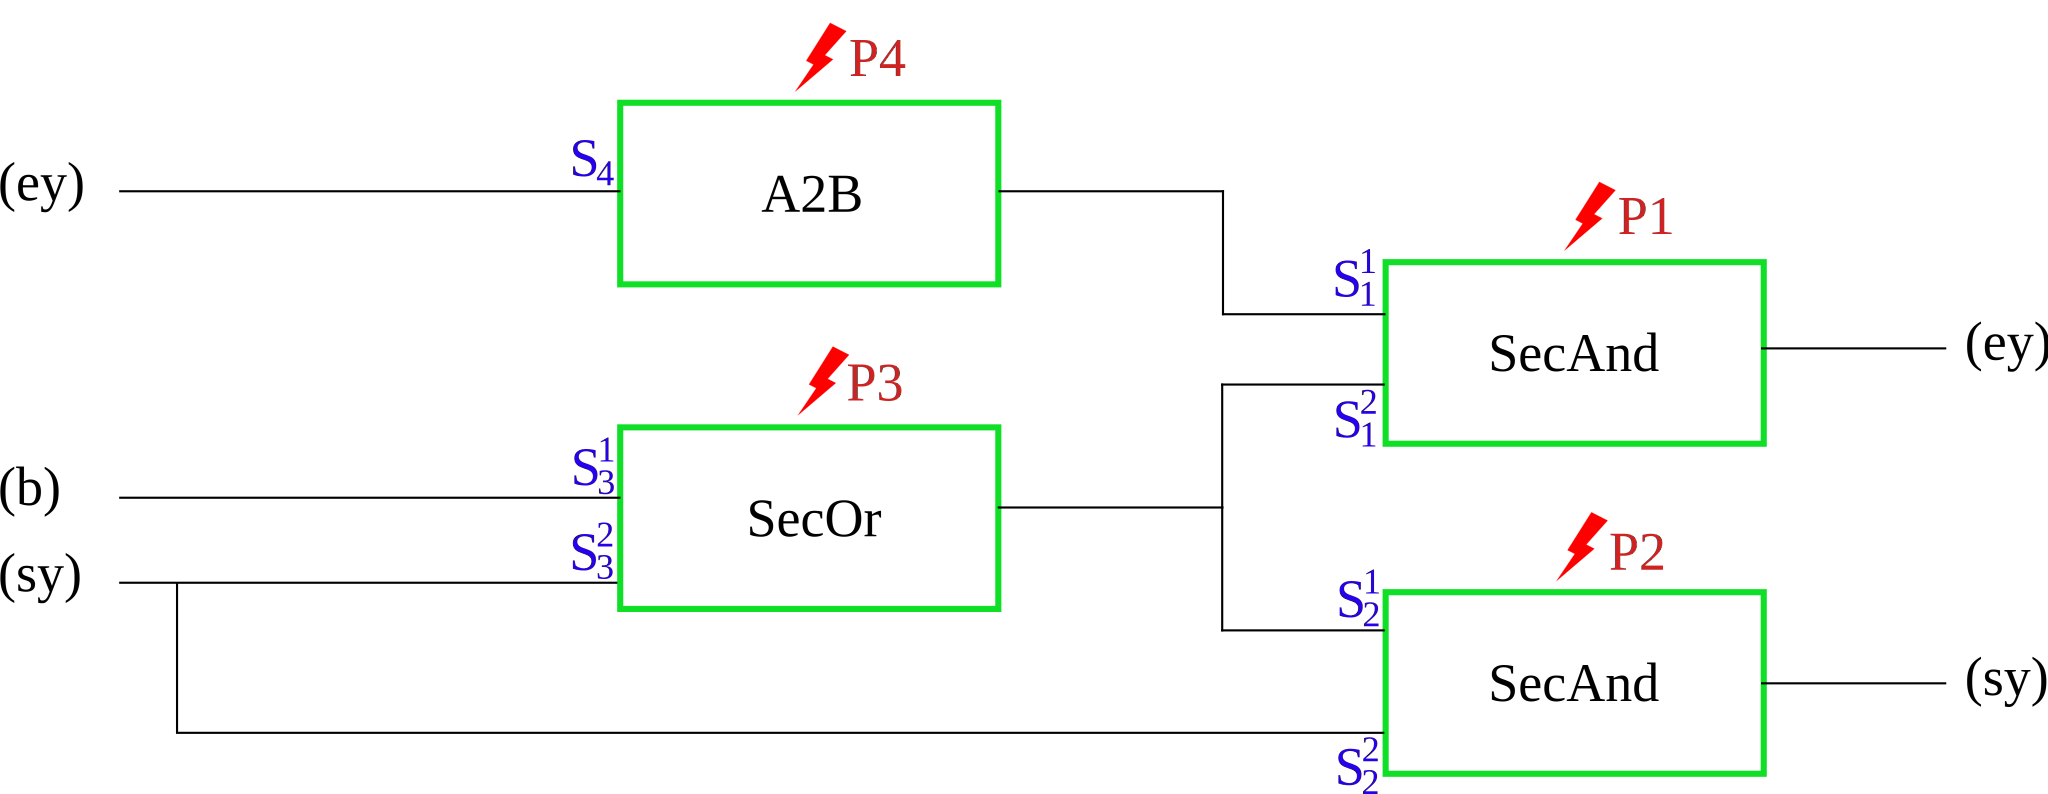
\includegraphics[width=7cm]{figure/SetExZero2.pdf}
  \label{fig:SetExponentZero}
  \caption{Abstract diagram of SetExponentZero}
\end{figure}
\begin{proof}
  We use an abstract diagram in Figure \ref{fig:SetExponentZero} for our demonstration. The gadget only contains \emph{t-SNI} gadgets and the input shares are distinct from the output shares for each gadgets. By composition of \emph{t-SNI} gadgets and independence of input and output shares, \textbf{SetExponentZero$_{floor}$} is itself \emph{t-SNI}.
\end{proof}

\begin{lemma}
  The gadget \textbf{SecFprUrsh$_\text{floor}$} (Algorithm \ref{algo:SecFprUrsh}) is \emph{t-SNI} secure.
\end{lemma}

\begin{figure}[!ht]
  \centering
  \includegraphics[width=7cm]{figure/secfprurshmod.png}
  \label{fig:Secfprurshmod}
  \caption{Abstract diagram of SecFprUrsh$_{floor}$}
\end{figure}

\begin{proof}
  The gadget \textbf{SecFprUrsh$_\text{floor}$} is a slight modification of the gadget \textbf{SecFprUrsh} from \cite{Chen_Chen_2024}. Ours does not compute the sticky bit but retains the rotated out information. We rely on their proof regarding the \emph{t-SNI} security of the gadget \textbf{Rotate} (see \cite{Chen_Chen_2024}, Lemma 3 and Figure 2). We now show that the operations following the rotation loop are \emph{t-SNI} secure. We use an abstract diagram in Figure \ref{fig:Secfprurshmod} for the demonstration. Let an adversary probe the intermediate values sets $\textcolor{red}{P_1}$ of \textbf{SecAnd}, $\textcolor{red}{P_2}$ of \textbf{SecAnd} and $\textcolor{red}{P_3}$ of \textbf{XOR}. As \textbf{SecAnd} is \emph{t-SNI} secure, one can use the sets \textcolor{blue}{$S_2^1$},\textcolor{blue}{$S_2^2$} (resp. \textcolor{blue}{$S_1^1$},\textcolor{blue}{$S_1^2$}) to simulate \textcolor{red}{$P_2$} (resp. \textcolor{red}{$P_1$}) and the ouput shares of $(rot)$ (resp. $(xi)>>(ci)$) with sizes no more than \textcolor{red}{$P_2$} (resp. \textcolor{red}{$P_1$}). One can simulate the probing set of \textcolor{red}{$P_3$} in the \textbf{XOR} and the simulation sets \textcolor{blue}{$S_2^2$} and \textcolor{blue}{$S_1^2$} with the output shares \textcolor{blue}{$S_3$} of the rotation of $(mi)$. All probes are now simulated with output shares \textcolor{blue}{$S_1^1\cup S_2^1$} of the rotation of $(xi)$ and \textcolor{blue}{$S_3$} of the rotation of $(mi)$. We have $\textcolor{blue}{|S_1^1\cup S_2^1|} \leq \textcolor{red}{|P_1| + |P_2|}$ and $\textcolor{blue}{|S_3|}\leq \textcolor{red}{|P_3|}+\textcolor{blue}{|S_2^2| + |S_1^2|} \leq \textcolor{red}{|P_3|+|P_2|+|P_1|}$. Along with the internal probes \textcolor{red}{$P_5$} and \textcolor{red}{$P_4$} into the rotation loop, can be simulated by input shares due to the \emph{t-SNI} security showed at first in (\cite{Chen_Chen_2024}, Lemma 3).
\end{proof}

\subsection{RemoveDecimal$_\text{floor}$}

FAIRE LA PREUVE

\begin{lemma}\label{lemma:remdec}
  The gadget \textbf{RemoveDecimal$_\text{floor}$} (Algorithm \ref{algo:RemoveDecimal_floor}) is \emph{t-SNI} secure.
\end{lemma}

\begin{figure}[!ht]
  \centering
  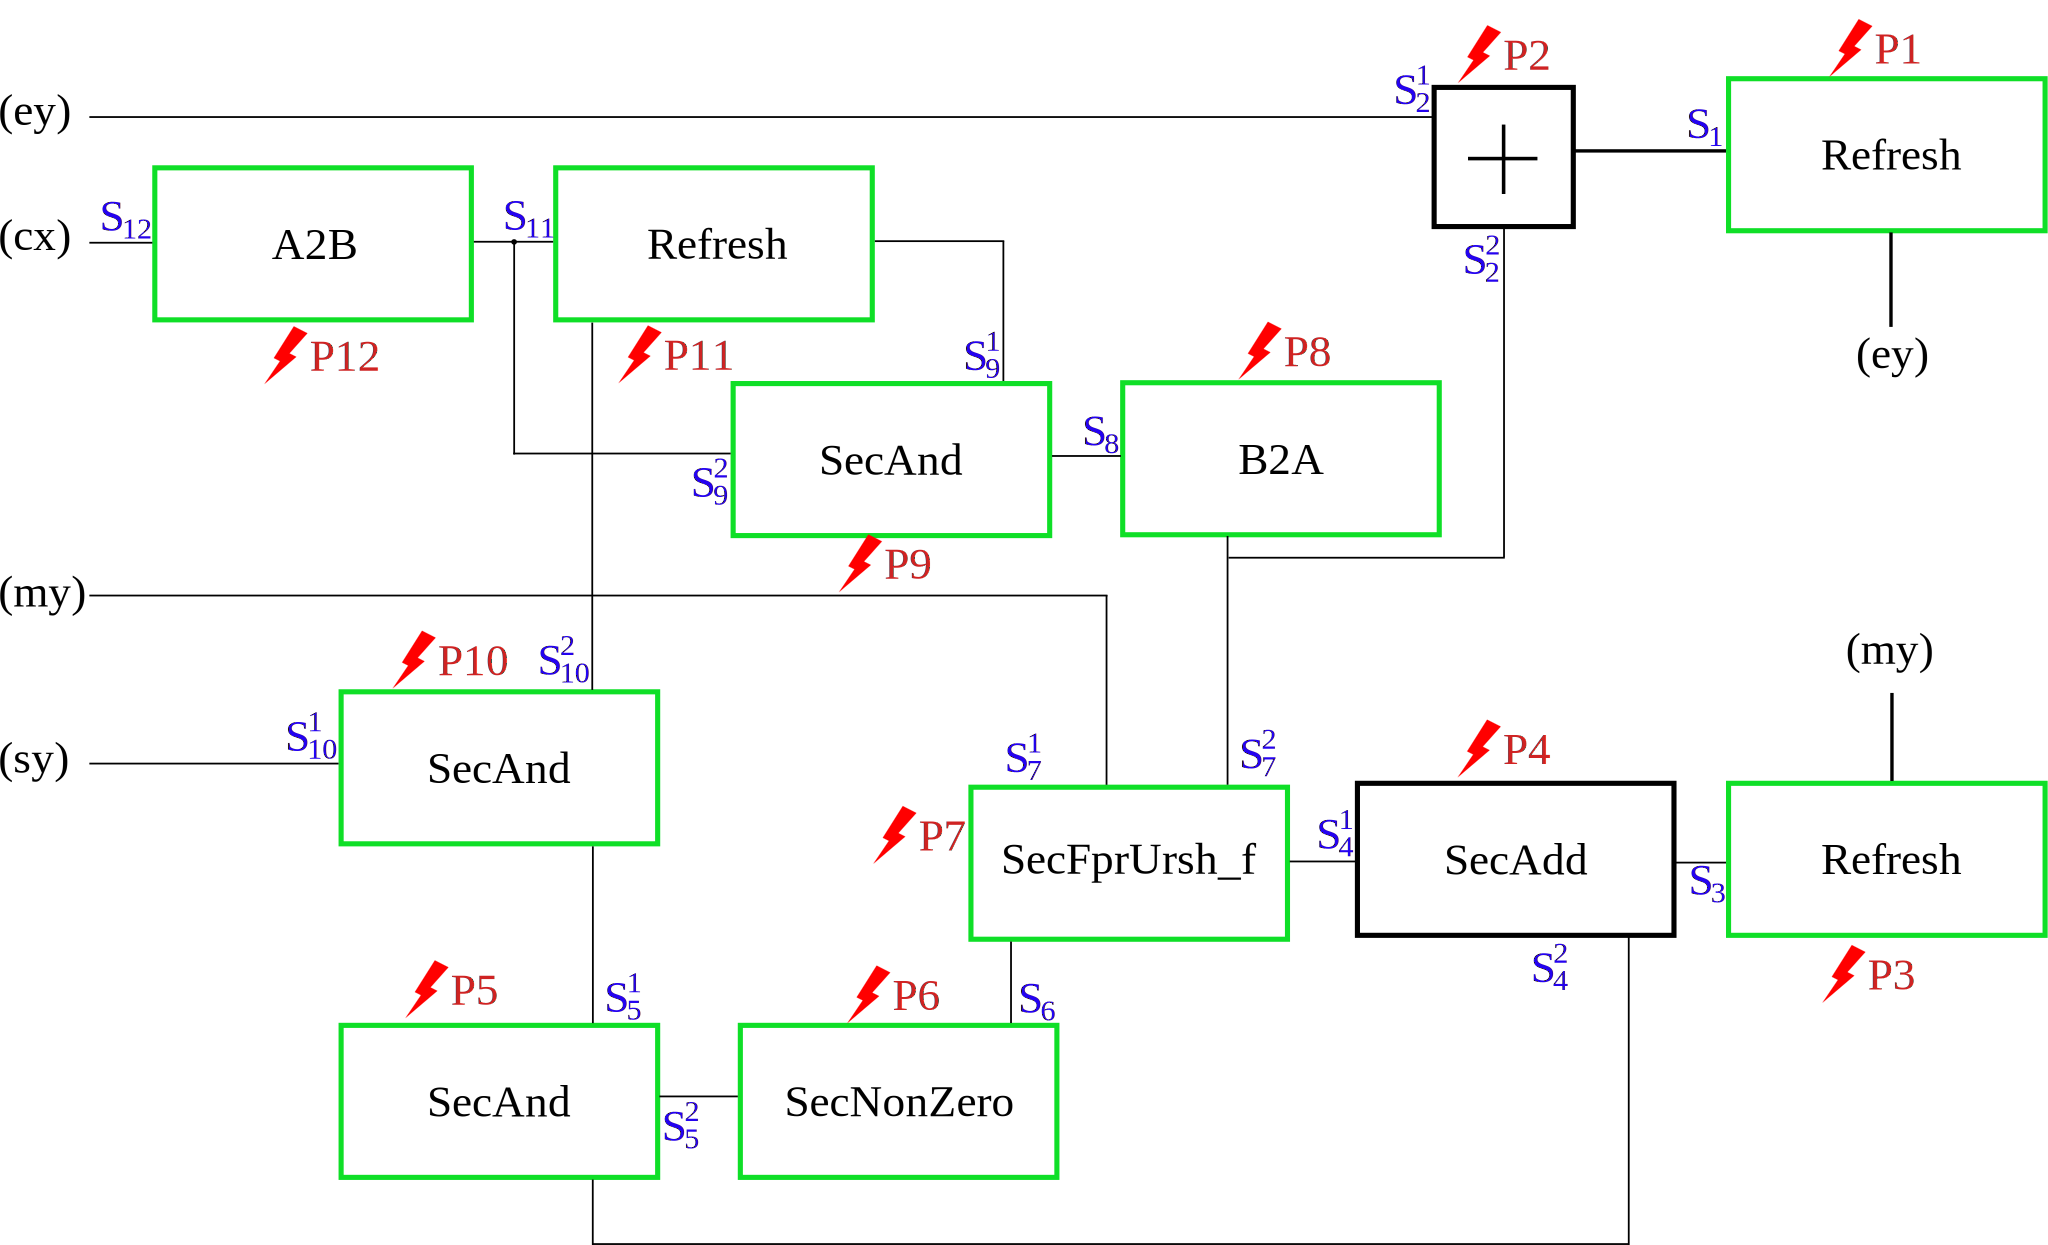
\includegraphics[width=8cm]{figure/RemoveDec2.pdf}
  \label{fig:RemoveDec}
  \caption{Abstract diagram of RemoveDecimal$_\text{floor}$}
\end{figure}
\begin{proof}
  We use an abstract diagram in Figure \ref{fig:RemoveDec} for the demonstration. Let assume an adversary probe the intermediate values sets of the output shares \textcolor{red}{$O$} and \textcolor{red}{$P_i$} in each gadget for $i\in\llbracket 1;12 \rrbracket$. We use simulation sets \textcolor{blue}{$S_i^j$} to simulate the values for each gadget. \emph{t-SNI} security implies that if the size of all probing sets $P_i$ is $t_I\leq t$ and if the size of values required to simulate in each gadget is smaller than $t$, then the simulation sets linked to the input shares are not bigger than $t_I$. \emph{t-SNI} gadgets imply $\textcolor{blue}{|S|} \leq \textcolor{red}{|P|}$ while \emph{t-NI} gadgets imply $\textcolor{blue}{|S|} \leq \textcolor{red}{|P|+|O|}$. As \textbf{Refresh}, \textbf{SecAnd}, \textbf{SecNonZero}, \textbf{SecFprUrsh$_{floor}$}, \textbf{B2A} and \textbf{A2B} are all \emph{t-SNI} secure while \textbf{SecAdd} and \textbf{$+$} are \emph{t-NI} secure, we can sequentially derive the following:
  \begin{multicols}{2}
    \begin{itemize}
      \item $\textcolor{blue}{|S_1|} \leq \textcolor{red}{|P_1|}$
      \item $\textcolor{blue}{|S_2^1|,|S_2^2|} \leq \textcolor{red}{|P_2|} + \textcolor{blue}{|S_1|} \leq \textcolor{red}{|P_2|+|P_1|}$
      \item $\textcolor{blue}{|S_3|} \leq \textcolor{red}{|P_3|}$
      \item $\textcolor{blue}{|S_4^1|,|S_4^2|} \leq \textcolor{red}{|P_4|} + \textcolor{blue}{|S_3|} \leq \textcolor{red}{|P_4|+|P_3|}$
      \item $\textcolor{blue}{|S_5^1|,|S_5^2|} \leq \textcolor{red}{|P_5|}$
      \item $\textcolor{blue}{|S_6|} \leq \textcolor{red}{|P_6|}$
      \item $\textcolor{blue}{|S_7^1|,|S_7^2|} \leq \textcolor{red}{|P_7|}$
      \item $\textcolor{blue}{|S_8|} \leq \textcolor{red}{|P_8|}$
      \item $\textcolor{blue}{|S_9^1|,|S_9^2|} \leq \textcolor{red}{|P_9|}$
      \item $\textcolor{blue}{|S_{10}^1|,|S_{10}^2|} \leq \textcolor{red}{|P_{10}|}$
      \item $\textcolor{blue}{|S_{11}|} \leq \textcolor{red}{|P_{11}|}$
      \item $\textcolor{blue}{|S_{12}|} \leq \textcolor{red}{|P_{12}|}$
    \end{itemize}
  \end{multicols}
  Based on the previous inequalities, one can check that no gadget requires more than $t_I$ values to be simulated. This apply to the input shares as well, with $\textcolor{blue}{|S_{10}^1|}\leq\textcolor{red}{|P_10|}$ for $(sy)$, $\textcolor{blue}{|S_7^1|}\leq\textcolor{red}{|P_7|}$ for $(my)$, $\textcolor{blue}{|S_12|} \leq \textcolor{red}{|P_12|}$ for $(cx)$ and $\textcolor{blue}{|S_2^1|}\leq\textcolor{red}{|P_2|} + \textcolor{blue}{|S_1|} \leq \textcolor{red}{|P_2| + |P_1|}$ for $(ey)$, no sizes being more than $t_I$.
\end{proof}

\begin{theorem}
  The gadget \textbf{SecBaseInt$_\text{floor}$} (Algorithm \ref{algo:SecFprBaseInt}) is \emph{t-SNI} secure.


\begin{figure}[!ht]
  \centering
  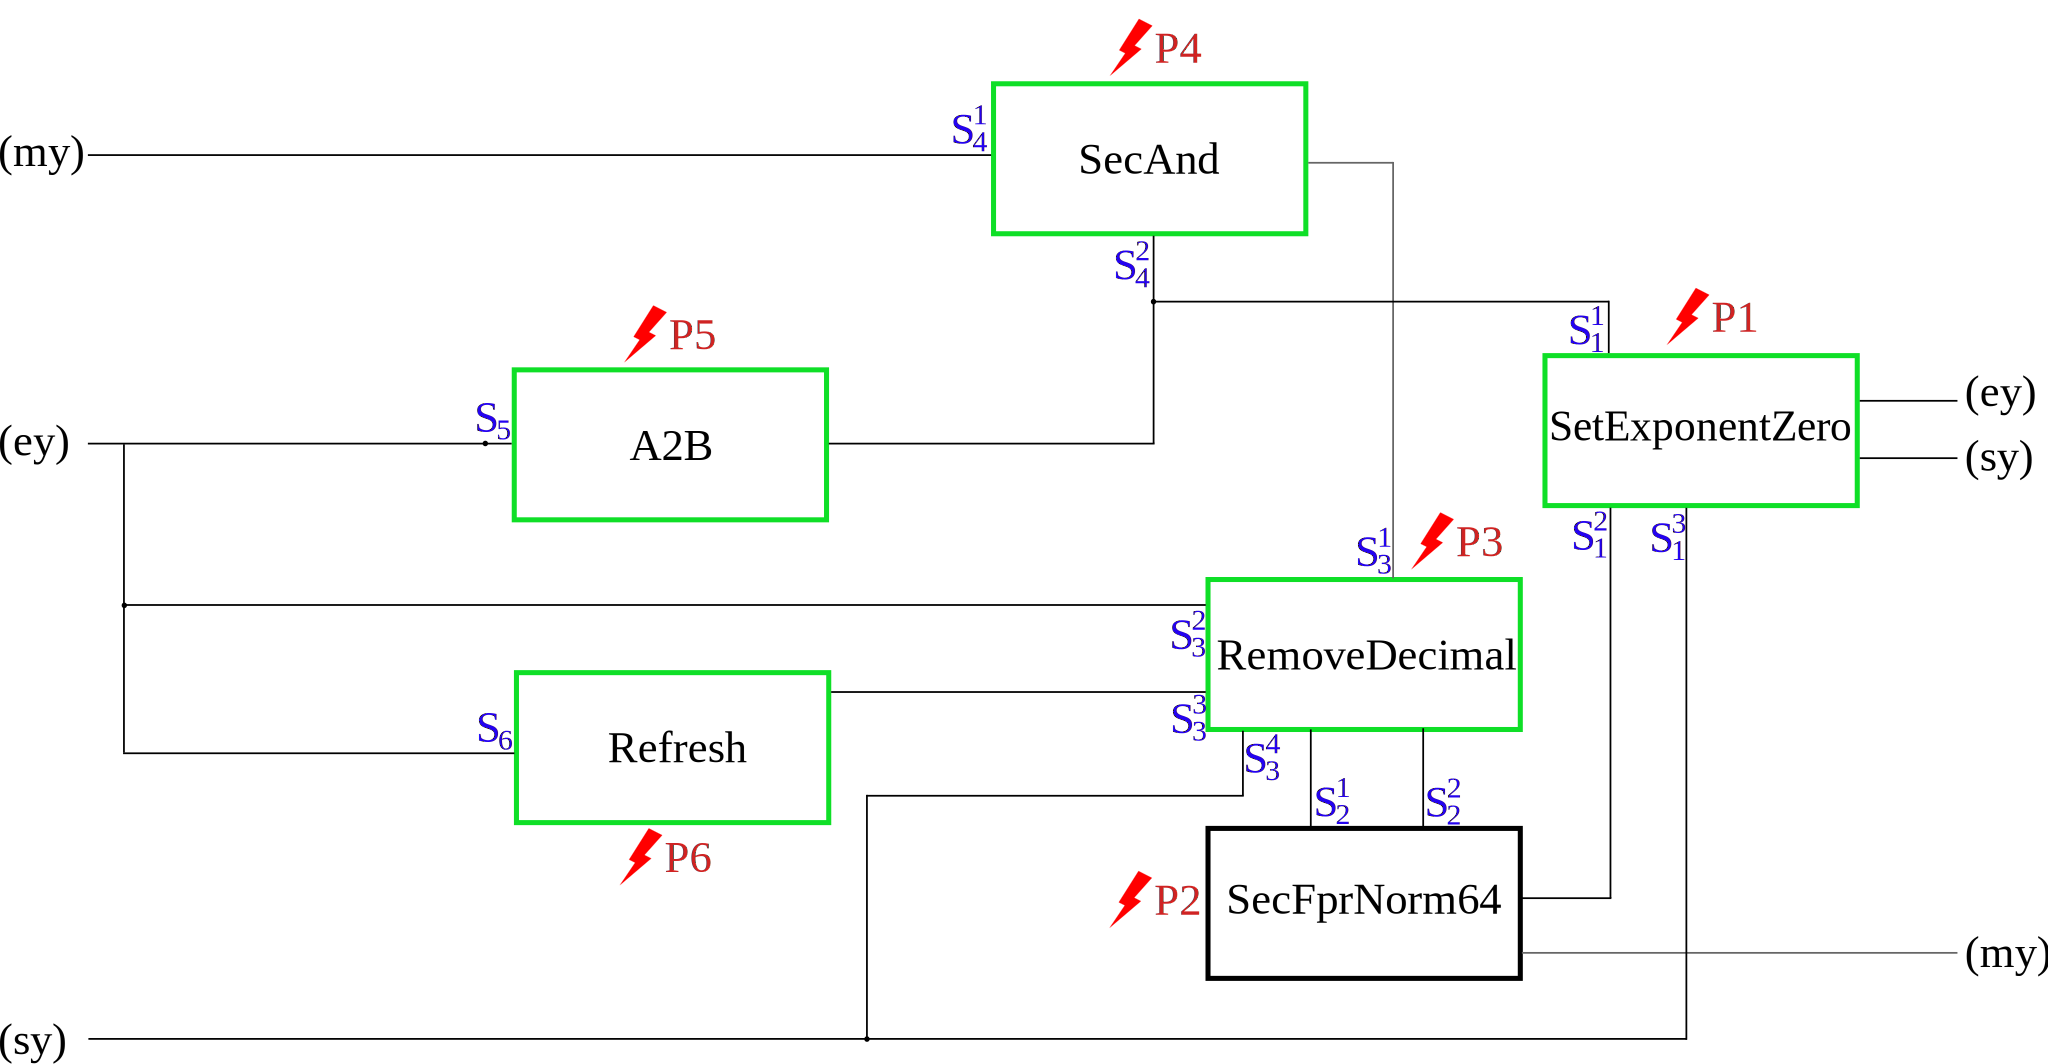
\includegraphics[width=10cm]{figure/secbaseint2.pdf}
  \label{fig:secbaseint}
  \caption{Abstract diagram of SecBaseInt$_\text{floor}$}
\end{figure}
\end{theorem}

\begin{proof}
  We use the same method as for the demonstration of Lemma \ref{lemma:remdec}. We use an abstract diagram in Figure \ref{fig:secbaseint} for the demonstration. Let assume an adversary probe the intermediate values sets of the output shares \textcolor{red}{$O$} and \textcolor{red}{$P_i$} in each gadget for $i\in\llbracket 1;6 \rrbracket$. We use simulation sets \textcolor{blue}{$S_i^j$} to simulate the values for each gadget. \emph{t-SNI} security implies that if the size of all probing sets $P_i$ is $t_I\leq t$ and if the size of values required to simulate in each gadget is smaller than $t$, then the simulation sets linked to the input shares are not bigger than $t_I$. As \textbf{SetExponentZero}, \textbf{RemoveDecimal}, \textbf{SecAnd}, \textbf{A2B} and \textbf{Refresh} are all \emph{t-SNI} secure while \textbf{SecFprNorm64} is \emph{t-NI} secure, we can sequentially derive the following:
  \begin{multicols}{2}
    \begin{itemize}
      \item $\textcolor{blue}{|S_1^1|,|S_1^2|,|S_1^3} \leq \textcolor{red}{|P_1|}$
      \item $\textcolor{blue}{|S_2^1|,|S_2^2|} \leq \textcolor{red}{|P_2| +|O_{(my)}|} $
      \item $\textcolor{blue}{|S_3^1|,|S_3^2|,|S_3^3|,|S_3^4|} \leq \textcolor{red}{|P_3|}$
      \item $\textcolor{blue}{|S_4^1|,|S_4^2|} \leq \textcolor{red}{|P_4|}$
      \item $\textcolor{blue}{|S_5|} \leq \textcolor{red}{|P_5|}$
      \item $\textcolor{blue}{|S_6|} \leq \textcolor{red}{|P_6|}$
    \end{itemize}
  \end{multicols}
  Based on the previous inequalities, one can check that no gadget requires more than $t_I$ values to be simulated. This also apply to the input shares, with $\textcolor{blue}{|S_{4}^1|}\leq\textcolor{red}{|P_4|}$ for $(my)$, $\textcolor{blue}{|S_5 \cup S_3^2\cup S_6|}\leq\textcolor{red}{|P_5|+|P_3| + |P_6|}$ for $(ey)$ and $\textcolor{blue}{|S_3^4\cup S_1^3|}\leq\textcolor{red}{|P_3|+|P_1|}$ for $(sy)$, none being more than $t_I$.
\end{proof}

\section{Application to FALCON}\label{sec:appfalcon}
\subsection{Masked Floor Function For FALCON}
\subsection{Masking the Gaussian Sampler}
\section{Performances}\label{sec:perf}



\section{Conclusion}\label{sec:conclusion}
\subsubsection{Acknowlegdments}

%
% ---- Bibliography ----
%
% BibTeX users should specify bibliography style 'splncs04'.
% References will then be sorted and formatted in the correct style.
%

\newpage


 \bibliographystyle{splncs04}
 \bibliography{falcon}

 \appendix
\section{Alternate Algorithms For Truncate and Rounding}\label{app:function}

\section*{Appendix}
\subsection*{Extract}

\begin{algorithm}[H]
  \caption{SecFprExtract(x)}
  \label{algo:SecFprExtract }
  \KwData{64-bit boolean shares $(x_i)_{1\leq i \leq n}$ for value x}
  \KwResult{64-bit boolean shares $(mx_i)_{1\leq i \leq n}$ for mantissa value mx; \\
            16-bit arithmetic shares $(ex_i)_{1\leq i \leq n}$ for exponent value ex; \\
            1-bit boolean shares $(sx_i)_{1\leq i \leq n}$ for sign value s.} 
  $(mx_i) \leftarrow (x_i^{[52:1]})$\;
  $(mx_i) \leftarrow$ SecAdd$((mx_i), (2^{52}, 0, \cdots, 0))$\tcp*{add implicit bit in the mantissa} 
  $(ex_i) \leftarrow (x_i^{[63:53]})$\;
  $(ex_i) \leftarrow$ B2A($(ex_i)$)\;
  $(sx_i) \leftarrow (x_i^{(64)})$\;
\Return{$((mx_i), (ex_i), (sx_i))$}\;
\end{algorithm}

\newpage
\subsection*{Truncature Function: Gadgets}

\begin{algorithm}
  \caption{RemoveDecimal$_{\text{trunc}}((my_i), (ey_i), (sy_i), (cx_i))$}
  \KwData{64-bit boolean shares $(my_i)_{1\leq i \leq n}$ for mantissa value my; \\
  16-bit arithmetic shares $(ey_i)_{1\leq i \leq n}$ for exponent value ey; \\
  1-bit boolean shares $(sy_i)_{1\leq i \leq n}$ for sign value sy\\
  16-bit arithmetic shares $(cx_i)_{1\leq i \leq n}$ for value cx = ex-2013.}
  \KwResult{64-bit boolean shares $(my_i)_{1\leq i \leq n}$ for mantissa value $my >> (52 - cx)$; \\
            16-bit arithmetic shares $(ey_i)_{1\leq i \leq n}$ for exponent value $ey +(52 - cx)$;} 
  $cx_1 \leftarrow cx_1 - 52$\tcp*{check if 0$\leq$c$<$51}
  $(c_i) \leftarrow$ A2B($(cx_i)$)\;
  $(cp_i) \leftarrow (c_i^{(16)})$\;
  $(cp_i) \leftarrow$ SecNonZero($cp_i$)\;
  $(c'_i) \leftarrow (- cp_i)$\tcp*{if cp = 0 cx = 0. if not cx = cx }
  $(c_i) \leftarrow$ SecAnd($(c_i), (cp_i)$)\;
  $(cx_i) \leftarrow$ B2A($(c_i)$)\;
  $(cd_i) \leftarrow (-cx_i)$\;
  $(my_i) \leftarrow$ SecFprUrsh$_f$($(my_i), (cd_i)$)\tcp*{$my >> 52 - cx$}
  $(ey_i) \leftarrow (ey_i + cd_i)$\; 
\Return{$((my_i), (ey_i))$}\;
\end{algorithm}



\begin{algorithm}[H]
  \caption{SetExponentZero$_{\text{trunc}}((ey_i), (sy_i), (b_i))$}
  \KwData{ 16-bit arithmetic shares $(ey_i)_{1\leq i \leq n}$ for exponent value ey; \\
  1-bit boolean shares $(sy_i)_{1\leq i \leq n}$ for sign value sy\\
  64-bit boolean shares $(b_i)_{1\leq i \leq n}$.}
  \KwResult{16-bit boolean shares $(ey_i)_{1\leq i \leq n}$ for exponent value $ey +(52 - cx)$;\\
            1-bit boolean shares $(sy_i)_{1\leq i \leq n}$ for sign value.} 
  
    $(ey_i) \leftarrow$ A2B($(ey_i)$)\;
    %$(b'_i) \leftarrow (-sy_i)$\;
    $(ey_i) \leftarrow$ SecAnd($(ey_i, b_i)$)\;
    $(sy_i) \leftarrow$ SecAnd($(sy_i, b_i)$)\;

\Return{$((ey_i), (sy_i))$}\;
\end{algorithm}



\newpage
\subsection*{Round Function: Gadgets}

\begin{algorithm}[H]
  \caption{RemoveDecimal$_{\text{round}}((my_i), (ey_i), (sy_i), (cx_i))$}
  \KwData{64-bit boolean shares $(my_i)_{1\leq i \leq n}$ for mantissa value my; \\
  16-bit arithmetic shares $(ey_i)_{1\leq i \leq n}$ for exponent value ey; \\
  1-bit boolean shares $(sy_i)_{1\leq i \leq n}$ for sign value sy\\
  16-bit arithmetic shares $(cx_i)_{1\leq i \leq n}$ for value cx = ex-2013.}
  \KwResult{64-bit boolean shares $(my_i)_{1\leq i \leq n}$ for mantissa value $my >> (52 - cx)$; \\
            16-bit arithmetic shares $(ey_i)_{1\leq i \leq n}$ for exponent value $ey +(52 - cx)$;\\
            1-bit boolean shares $(Rnd_i)$ for value Rnd -- the bit at position -1.} 
  $cx_1 \leftarrow cx_1 - 53$\tcp*{check if 0$\leq$c$<$51}
  $(c_i) \leftarrow$ A2B($(cx_i)$)\;
  $(cp_i) \leftarrow (c_i^{(16)})$\;
  $(cp_i) \leftarrow$ SecNonZero($cp_i$)\;
  $(rshORnot_i) \leftarrow (-cp[i])$\; 
  $(c'_i) \leftarrow (- cp_i)$\tcp*{if cp = 0 cx = 0. if not cx = cx }
  $cx_1 \leftarrow cx_1 + 1$\;
  $(c_i) \leftarrow$ A2B($(cx_i)$)\;
  $(c_i) \leftarrow$ SecAnd($(c_i), (cp_i)$)\;
  $(cx_i) \leftarrow$ B2A($(c_i)$)\;
  $(cd_i) \leftarrow (-cx_i)$\;
  $(my_i) \leftarrow$ SecFprUrsh($(my_i), (cd_i)$)\tcp*{$my >> 53 - cx$}
  $(Rnd_i) \leftarrow (my_i^{(1)})$\;
  $(Rnd_i) \leftarrow$ SecNonZero$(Rnd_i)$\;
  $(Rnd_i) \leftarrow$ SecAnd($(Rnd_i), (rshORnot_i)$)\;
  $(my1_i) \leftarrow$ $(my_i)>>1$ , $\quad (e1_i) \leftarrow$ $(1,0,\cdots, 0)$\;
  $(my2_i) \leftarrow$ $(my_i)\qquad \quad$,  $\quad(e2_i) \leftarrow$ $(0,\cdots, 0)$\;
  $(my1_i) \leftarrow$ SecAnd($(my1_i), (rshORnot_i))\quad $, $(e1_i) \leftarrow$ SecAnd($(e1_i), (rshORnot_i)$)\;
  $(rshORnot_i) \leftarrow (-rshORnot_i)$\;
  $(my2_i) \leftarrow$ SecAnd($(my2_i), (rshORnot_i))\quad $, $(e2_i) \leftarrow$ SecAnd($(e2_i), (rshORnot_i)$)\;
  $(my_i) \leftarrow$ SecOr($(my1_i), (my2_i)$)\;
  $(my_i) \leftarrow$ SecAdd($(my_i), (Rnd_i)$)\;
  $(e1_i) \leftarrow$ SecOr($(e1_i), (e2_i)$)\;
  $(e1_i) \leftarrow$ B2A($(e1_i)$)\; 
  $(ey_i) \leftarrow (ey_i + e1_i) $\;
  $(ey_i) \leftarrow (ey_i + cd_i)$\; 
\Return{$((my_i), (ey_i), (Rnd_i))$}\;
\end{algorithm}

\begin{algorithm}[H]
  \caption{SetExponentZero$_{\text{round}}((ey_i), (sy_i), (b_i), (Rnd_i))$}
  \KwData{ 16-bit arithmetic shares $(ey_i)_{1\leq i \leq n}$ for exponent value ey; \\
  1-bit boolean shares $(sy_i)_{1\leq i \leq n}$ for sign value sy\\
  64-bit boolean shares $(b_i)_{1\leq i \leq n}$.}
  \KwResult{16-bit boolean shares $(ey_i)_{1\leq i \leq n}$ for exponent value $ey +(52 - cx)$;\\
            1-bit boolean shares $(sy_i)_{1\leq i \leq n}$ for sign value.} 
  
    $(ey_i) \leftarrow$ A2B($(ey_i)$)\;
    $(b'_i) \leftarrow (Rnd_i)$\;
    $(b'_i) \leftarrow$ SecOr($(b'_i), (b_i)$)\;
    $(ey_i) \leftarrow$ SecAnd($(ey_i, b'_i)$)\;
    $(sy_i) \leftarrow$ SecAnd($(sy_i, b'_i)$)\;

\Return{$((ey_i), (sy_i))$}\;
\end{algorithm}

\end{document}
